% ============================================================
% Amazon-VT CFP 2026-2027 — 1-Page Abstract v4d
% AKG-E Synthesis: domain-agnostic framing (v4) + VVUQ backbone (v4b)
%   + BIM/IFC+FEA depth (v4c) + engineering-agent citations (deep research)
% Primary: AI Accelerated Science & Engineering
% Secondary: Agentic AI
% Format: IEEE 2-column
% ============================================================

\documentclass[conference, 10pt]{IEEEtran}

\usepackage[utf8]{inputenc}
\usepackage[T1]{fontenc}
\usepackage{graphicx}
\usepackage{hyperref}
\usepackage{microtype}
\usepackage{cite}
\usepackage{enumitem}
\setlist{nosep, leftmargin=1.5em, topsep=0.2em}
\usepackage{tikz}
\usetikzlibrary{positioning, arrows.meta, shapes.geometric, fit, calc}

\title{Agentic Knowledge Graphs for AI-Accelerated Engineering\\with Generalizable Simulation-in-the-Loop Validation}
\author{}
\date{}

% ============================================================
\begin{document}

\maketitle
\thispagestyle{empty}

\vspace{-1.5em}

\noindent\textbf{Primary Topic:} AI Accelerated Science \& Engineering \hfill
\textbf{Secondary:} Agentic AI

\vspace{0.5em}

AI-driven breakthroughs---from biomolecular structure prediction~\cite{Abramson2024AlphaFold3} to materials discovery~\cite{Merchant2023GNoME}---show that tightly coupling domain knowledge with simulation dramatically accelerates scientific progress. Engineering disciplines face an analogous opportunity, yet large language models (LLMs) remain poorly suited to engineering practice: they hallucinate physical quantities~\cite{Ji2023HallucinationSurvey}, cannot enforce constraint satisfaction, and lack grounding in the structured ontologies and simulation feedback loops that define engineering workflows. Crucially, although Verification, Validation, and Uncertainty Quantification (VVUQ)~\cite{Oberkampf2010VVUQ} is well-established for validating computational simulation models, \textit{no methodology exists for systematically validating AI agent-generated engineering outputs}---a trust gap that blocks deployment. Emerging engineering-agent work---including multi-agent LLM frameworks for finite element analysis~\cite{LLMAgentsFEM2025} and self-correcting multi-agent physics simulation~\cite{Park2026MCPSIM}---confirms both the opportunity and the open validation challenge.

This project proposes \textbf{Agentic Knowledge Graph Engineering (AKG-E)}, a domain-agnostic framework in which LLM-powered agents reason over structured engineering knowledge, invoke physics-based simulations, and validate outputs through VVUQ. AKG-E applies three shared layers uniformly across engineering domains---with only the domain KG and simulator swapped: (1)~a \textit{domain ontology layer} encoding engineering KGs with entities, constraints, physical laws, and design rules; (2)~a \textit{simulation integration layer} exposing domain tools (FEA solvers~\cite{Logg2012FEniCS}, microsimulators) as typed agent-callable interfaces; and (3)~a \textit{VVUQ validation layer} that verifies agent-generated designs against physical laws, quantifies prediction uncertainty via Monte Carlo propagation through agent pipelines, and enforces regulatory constraints. Agents orchestrate across retrieval-augmented generation~\cite{Lewis2020RAG}, structured graph queries~\cite{Edge2024GraphRAG}, and simulation calls.

\begin{figure}[t]
    \centering
    \resizebox{\columnwidth}{!}{%
    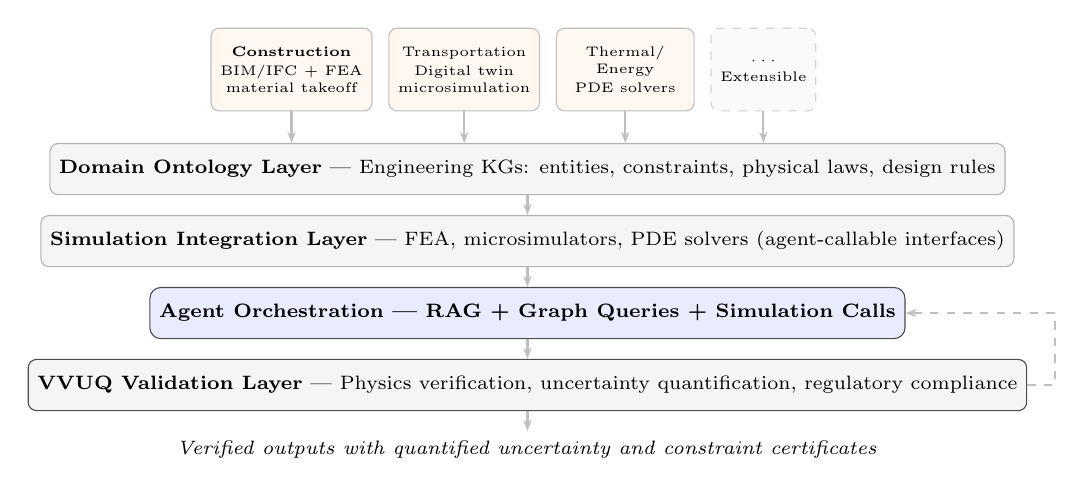
\begin{tikzpicture}[
        node distance=0.30cm and 0.20cm,
        layerbox/.style={rectangle, rounded corners=3pt, draw=gray!60, fill=gray!8, minimum width=7.8cm, minimum height=0.65cm, align=center, font=\scriptsize},
        dombox/.style={rectangle, rounded corners=3pt, draw=gray!50, fill=orange!6, minimum width=1.75cm, minimum height=1.05cm, align=center, font=\tiny},
        extbox/.style={rectangle, rounded corners=3pt, draw=gray!35, fill=gray!4, minimum width=1.05cm, minimum height=1.05cm, align=center, font=\tiny, dashed},
        agentbox/.style={rectangle, rounded corners=4pt, draw=black!70, fill=blue!8, minimum width=7.8cm, minimum height=0.65cm, align=center, font=\scriptsize\bfseries},
        arr/.style={-{Stealth[length=4pt]}, thick, gray!50},
    ]
        % Domain modules (top row)
        \node[dombox] (con) {\textbf{Construction}\\[1pt]BIM/IFC + FEA\\material takeoff};
        \node[dombox, right=0.20cm of con] (traf) {Transportation\\[1pt]Digital twin\\microsimulation};
        \node[dombox, right=0.20cm of traf] (therm) {Thermal/\\Energy\\[1pt]PDE solvers};
        \node[extbox, right=0.20cm of therm] (ext) {$\cdots$\\Extensible};

        % Domain ontology layer (centered under domain row)
        \node[layerbox, below=0.40cm of $(con.south)!0.5!(ext.south)$] (onto) {\textbf{Domain Ontology Layer} --- Engineering KGs: entities, constraints, physical laws, design rules};

        % Simulation integration layer
        \node[layerbox, below=0.25cm of onto] (sim) {\textbf{Simulation Integration Layer} --- FEA, microsimulators, PDE solvers (agent-callable interfaces)};

        % Agent orchestration
        \node[agentbox, below=0.25cm of sim] (agent) {Agent Orchestration --- RAG + Graph Queries + Simulation Calls};

        % VVUQ validation
        \node[layerbox, below=0.25cm of agent, draw=black!70] (val) {\textbf{VVUQ Validation Layer} --- Physics verification, uncertainty quantification, regulatory compliance};

        % Output
        \node[font=\scriptsize, below=0.25cm of val] (out) {\textit{Verified outputs with quantified uncertainty and constraint certificates}};

        % Arrows: domain boxes to onto
        \draw[arr] (con.south) -- (con.south |- onto.north);
        \draw[arr] (traf.south) -- (traf.south |- onto.north);
        \draw[arr] (therm.south) -- (therm.south |- onto.north);
        \draw[arr] (ext.south) -- (ext.south |- onto.north);

        % Layer arrows
        \draw[arr] (onto) -- (sim);
        \draw[arr] (sim) -- (agent);
        \draw[arr] (agent) -- (val);
        \draw[arr] (val) -- (out);

        % Feedback loop
        \draw[arr, dashed] (val.east) -- ++(0.35,0) |- (agent.east);
    \end{tikzpicture}
    }%
    \caption{\textbf{AKG-E Domain-Agnostic Architecture.} Domain modules (Construction: primary pilot; Transportation, Thermal/Energy: planned extensions) plug into shared ontology, simulation, and VVUQ layers. Only the domain KG and simulator module are swapped across domains; agent orchestration and VVUQ validation are reused unchanged. Dashed arrow: VVUQ feedback drives iterative refinement.}
    \label{fig:framework}
    \vspace{-0.5em}
\end{figure}

This research pursues two questions: \textbf{RQ1:} How can VVUQ methodology be adapted to validate AI agent-generated engineering outputs, providing quantified uncertainty bounds and enforceable physical and regulatory constraints? \textbf{RQ2:} Does a domain-agnostic AKG-E architecture yield measurable constraint violation reductions across engineering domains relative to LLM-only and RAG-only baselines? These questions address a gap that existing engineering-agent work~\cite{Park2026MCPSIM,LLMAgentsFEM2025} has not yet closed: a rigorous, reusable validation layer. The intellectual merit is the \textit{first principled VVUQ methodology for agentic AI outputs} and a generalizable architecture that separates domain-specific knowledge from shared reasoning and validation logic.

The primary pilot is \textbf{construction engineering}: agents parse BIM/IFC~\cite{Eastman2011BIM} models, perform automated material takeoff, execute structural verification via FEA~\cite{Logg2012FEniCS}, and flag schedule conflicts---all gated through VVUQ. Construction digital twin research~\cite{Soman2025ConstructionDT} motivates the trust thresholds for autonomous-versus-human-reviewed decisions. Expandability is explicit: the same three layers apply to \textbf{transportation engineering} (digital twin simulation~\cite{Tao2019DigitalTwin}, traffic microsimulation) and \textbf{thermal/energy engineering} (PDE-based solvers) by swapping only the domain KG and simulator module, with no changes to orchestration or VVUQ layers. The framework targets deployment via Amazon Bedrock Knowledge Bases~\cite{AWSBedrockHybridSearch2024}. We hypothesize $>$50\% constraint violation reduction versus unconstrained LLM baselines and calibrated uncertainty estimates (coverage within 10\% of nominal). Deliverables include an open AKG-E framework with pluggable domain KG templates, VVUQ benchmarks, and construction/transportation evaluation datasets---providing replicable evidence that \textbf{simulation-grounded agentic AI} outperforms unstructured LLM approaches for engineering decision-support.

\bibliographystyle{IEEEtran}
\bibliography{references}

\end{document}
